\subsubsection{先给 1440\texorpdfstring{$\times$}{×}1080@250 Hz 算笔账}
\label{sec:ros2-image-budget}
前面用字符串把收发流程跑通了，接下来换成我们实际工作中会碰到的图像。相机最高可以达到 $1440\times1080@250\,\mathrm{Hz}$（宽 $\times$ 高），也就是每隔 4 ms 来一帧。这个数字说的是相机的工作上限；接到 ROS2 后，采集、转换、传输和识别能不能一直跟上，还得分开测。你大概也不希望相机拍得飞快，识别节点却在认真处理半秒前的装甲板。

先把图像看成一块内存。每帧像素数是 $1440\times1080=1\,555\,200$，紧密排列时，原始像素负载率为
\[
  B=\text{宽}\times\text{高}\times\text{每像素字节数}\times\text{帧率}.
\]
这里使用十进制单位：$1\,\mathrm{MB}=10^6\,\mathrm{B}$，$1\,\mathrm{GB}=10^9\,\mathrm{B}$。表\ref{tab:ros2-image-budget} 只算像素，不含消息头、DDS 分片、协议开销或行尾填充。实际 \texttt{Image} 要核对 \texttt{step}，像素数组大小通常按 \texttt{step}$\times$\texttt{height} 计算；相机输出的打包格式也要先确认。

\begin{table}[htbp]
\centering
\caption{1440×1080、250 Hz 的紧密排列图像预算}
\label{tab:ros2-image-budget}
\begin{tabular}{lrrr}
\toprule
格式 & 每帧 / MB & 每秒 / MB & 纯像素 / Gbit/s\\
\midrule
mono8 / Bayer8 & 1.5552 & 388.8 & 3.1104\\
mono16 & 3.1104 & 777.6 & 6.2208\\
bgr8 / rgb8 & 4.6656 & 1166.4 & 9.3312\\
\bottomrule
\end{tabular}
\end{table}

\begin{example}[复制一帧，到底搬了多少东西]
假设相机先输出 Bayer8，我们在采集端转成 BGR8，再把完整彩色图像交给识别节点。一秒的 BGR8 像素就有约 1.17 GB。每多做一次完整复制，都要读一遍源数据、写一遍目标数据，按这个负载估算，新增的读写量约为 $2\times1.1664=2.3328\,\mathrm{GB/s}$。如果连续几段处理都各自复制一次，这笔账会不断叠加。

这个估算帮助我们定位值得优化的边界，不能当作内存总线实测值：缓存命中、写分配、DMA 和库实现都会改变真实流量。Bayer 转 BGR 本身也是一次产生新数据的处理，不能靠 \texttt{std::move} 把它省掉。跨机器时，千兆网连 mono8 的纯像素都装不下；BGR8 接近万兆网的标称带宽，还没有给协议和其他数据留足空间。应先规划分辨率、帧率、ROI、图像格式与网络，再挑中间件。
\end{example}

\paragraph*{队列深度救不了长期超时}
250 Hz 的到帧间隔是 4 ms；单个串行处理阶段若每帧要 8 ms，理想上限也只有 125 Hz。加大 \texttt{KeepLast} 深度可以吸收短时抖动，却不能提高长期处理能力。深度 5 的一份 BGR8 历史，仅像素就约 23.33 MB；多端历史和工作缓冲还会继续占内存。在 250 Hz 输入下，深度 10 对应约 40 ms 的入队跨度，这不是延迟上界；发布端阻塞、其他队列和调度等待都可能再增加图像年龄。

对于需要及时瞄准的识别链路，我们通常先用小深度、易于丢弃旧帧的策略作起点，例如兼容的 \texttt{best\_effort} 加 \texttt{KeepLast(1)} 或较小深度，再按丢帧与延迟实测调整。离线录制如果要求完整保存，就要另算存储吞吐和可靠传输成本，必要时降帧率或独立部署。可靠传输解决的是交付语义，不能把处理器的工作速度翻倍。

\begin{exercise}
\label{ex:v2-ros-image-budget}
计算该相机 Bayer8 和 BGR8 的负载率。若 BGR8 链路新增两次完整复制，估算新增读写量；再判断每帧串行处理 8 ms 时，把队列从 5 改成 100 能否持续处理全部 250 Hz 输入。说明你会同时记录哪两个指标，避免只看话题频率。
\end{exercise}

\subsubsection{中间件怎么选：先比较同一条链路}
\label{sec:ros2-rmw-selection}
\texttt{rclcpp} 下面的 RMW 是中间件接口，并不是某一家 DDS 产品的名字。Humble 的常用起点是 Fast DDS（\nolinkurl{rmw_fastrtps_cpp}），我们也可以换成 Cyclone DDS（\nolinkurl{rmw_cyclonedds_cpp}），或者使用基于 Zenoh 的 \nolinkurl{rmw_zenoh_cpp}。发布与订阅的基本代码通常不用跟着改，但发现机制、传输路径、缓存与配置方法会变化。小字符串测试能确认通信成立，大图像测试才能暴露吞吐、分片与排队问题。

\begin{center}
\begin{tabular}{p{0.17\textwidth}p{0.35\textwidth}p{0.35\textwidth}}
\toprule
实现 & 接入与发现 & 图像路径与评估重点\\
\midrule
Fast DDS & Humble 默认 RMW；按需使用自己的 XML 配置 & 同步/异步发布影响调用线程；共享内存传输与 Data Sharing 分开核对，默认未启用后者\\
Cyclone DDS & 安装对应 RMW 后切换；配置使用 \nolinkurl{CYCLONEDDS_URI} & 使用自己的传输与线程配置；本章借出探测为 false，不能套用 Fast DDS 的调优变量\\
Zenoh & 安装 \nolinkurl{rmw_zenoh_cpp}；默认通过路由器协助发现 & 同机 peer 可直接交换数据；共享内存需单独配置，不能把“使用 Zenoh”当作“已经零拷贝”\\
共同口径 & 两端使用相同 RMW、消息、QoS 与部署布局 & 一起看实际发送频率、接收比例、延迟尾部与资源占用，保留配置与原始日志\\
\bottomrule
\end{tabular}
\end{center}

切换操作见前面的环境小节。这里进一步要求两端显式设置同一种 RMW，停止旧节点后重启；试验使用独立域，避免遗留订阅者混进来。DDS 实现之间存在互操作能力，但当前实验应先排除混用实现造成的变量。尤其不要一边换 RMW、一边改可靠性和图像尺寸，最后凭“好像快了”给某一家颁奖。

\begin{example}[安排一个可以解释结果的对照]
本节与后两节共用 \path{examples/ros2/image-path-demo}。它生成同样的图像，先固定帧数、尺寸、频率、\texttt{best\_effort} 和深度 5，然后对两种 RMW 分别运行三种布局：两个进程、同一进程关闭进程内通信、同一进程开启进程内通信。这样，前两项帮助观察中间件与进程边界，最后一项帮助观察所有权传递；完整构建和命令在下一节。

结果至少一起看发送实际频率、接收比例和 P95/P99 延迟。P95 表示约 95\% 的已收到样本不超过这个延迟；丢掉的样本不在延迟统计中，因此低延迟也可能伴随大量丢帧。再记录 CPU 时间和内存作为辅助信息。在真正的系统选型前，至少重复几轮，补测实际相机、算法、录制和网络。
\end{example}

Fast DDS 的 RMW 默认项、同步与异步发布、Data Sharing 配置可查 \href{https://github.com/ros2/rmw_fastrtps/blob/humble/README.md}{Humble 分支说明}；需要调整网卡、发现与报文时，再查 \href{https://github.com/ros2/rmw_cyclonedds/blob/humble/README.md}{Cyclone DDS 的 ROS2 接口说明}。这些资料帮助你找到对应配置，最终选择仍要落在自己的链路数据上。

\paragraph*{把 Zenoh 接到同一条图像链路}
Zenoh 不是另一家 DDS。\texttt{rmw\_zenoh\_cpp} 把 ROS2 的中间件接口接到 Zenoh，所以我们仍然编写熟悉的节点、消息和组件，下面的发现与传输方式却换了。默认配置先连接本机 Zenoh 路由器，由它协助节点发现彼此；同机 peer 会建立直接连接，不能把它理解成“每帧图像都要绕路由器一圈”。需要跨主机、无线链路或多机器人通信时，可以进一步配置路由与连接拓扑，但这些条件还要另测。

\begin{example}[让 Zenoh 运行已有组件]
先完成下一节的 \path{image_path_demo} 构建，再回到这里操作。第一个终端在 Ubuntu 22.04/Humble 中安装接口并启动路由器：
\par\medskip\noindent\begin{minipage}{\linewidth}
\begin{tbash}
source /opt/ros/humble/setup.bash
sudo apt update
sudo apt install ros-humble-rmw-zenoh-cpp
ros2 run rmw_zenoh_cpp rmw_zenohd
\end{tbash}
\end{minipage}\par\smallskip
保持这个终端运行。第二个终端加载同一个组件工程，把 RMW 改为 Zenoh：
\par\medskip\noindent\begin{minipage}{\linewidth}
\begin{tbash}
source /opt/ros/humble/setup.bash
cd ~/image_path_ws
source install/setup.bash
export ROS_DOMAIN_ID=87
export ROS_LOCALHOST_ONLY=1
export RMW_IMPLEMENTATION=rmw_zenoh_cpp
ros2 launch image_path_demo path.launch.py mode:=intra
\end{tbash}
\end{minipage}\par\smallskip
默认仍是 64×48、25 Hz、100 帧。等 \texttt{SOURCE\_DONE} 后，先在第二个终端按 Ctrl+C 保存统计，再停止第一个终端的路由器。检查完整接收、\texttt{bad\_frames=0} 和进程内地址记录；这次节点源码没有改变。需要查询图时，查询终端也要加载同一工程、域和 RMW；可使用 \texttt{ros2 component list --no-daemon}，避免旧 RMW 的后台缓存混入结果。

若收不到消息，先查路由器是否启动、默认 7447 端口是否被占用、两端 RMW 和域是否一致，以及是否遗留 \texttt{ZENOH\_CONFIG\_OVERRIDE} 或自定义配置文件。这里两端都用 Humble；看得到远端节点不等于跨发行版消息能交付。Zenoh RMW 也不会自动与 DDS 节点或 \texttt{zenoh-bridge-ros2dds} 互通，桥接需要单独核对协议与部署。

停止手动实验后，可以直接让记录器管理每轮路由器并跑三种布局：
\par\medskip\noindent\begin{minipage}{\linewidth}
\begin{tbash}
python3 src/image_path_demo/compare.py \
  --output /tmp/image-path-zenoh-small \
  --rmws rmw_zenoh_cpp
\end{tbash}
\end{minipage}\par\smallskip
记录器使用自己的本机 17447 端口，启动前检查占用，退出时只关闭自己启动的路由器与节点；换端口用 \texttt{--zenoh-port}。默认仍不启用 Zenoh 共享内存。路由器的 CPU/RSS 也计入这一轮资源记录，不能遗漏它，再声称整个部署更省资源。
\end{example}

Zenoh 的发现、路由与参数可查 \href{https://github.com/ros2/rmw_zenoh/blob/humble/README.md}{Humble 安装与配置说明}和\href{https://github.com/ros2/rmw_zenoh/blob/humble/docs/design.md}{RMW 设计说明}。先把相同节点跑通，再测试大图像与实际网络，不能凭协议名字判断哪一个更快。

\begin{exercise}
\label{ex:v2-ros-rmw-choice}
运行下一节的小图像对照，找出 Fast DDS、Cyclone DDS 与 Zenoh 在 \texttt{separate} 模式下的发送频率、接收比例与 P95。列出本轮保持相同的条件，并说明 Zenoh 的路由器在本次实验中负责什么、如何正常停止。若其中一项更好，说明还需补测什么，才能决定实际相机使用哪个实现。
\end{exercise}

\subsubsection{零拷贝与组件容器：先管好图像的所有权}
\label{sec:ros2-image-components}
\textbf{零拷贝（zero-copy）一定要说清楚省掉哪一段复制。}我们先追求“相机发布节点到识别订阅回调”这一段的进程内像素传递：把两个节点装进同一个进程，让 \texttt{rclcpp} 直接交接消息的所有权。相机 SDK 向消息填数据、颜色转换、校正和 CPU/GPU 传输仍需分别检查。这一段省了复制，不等于整条采集与推理链路都没有复制。

\begin{figure}[H]
\centering
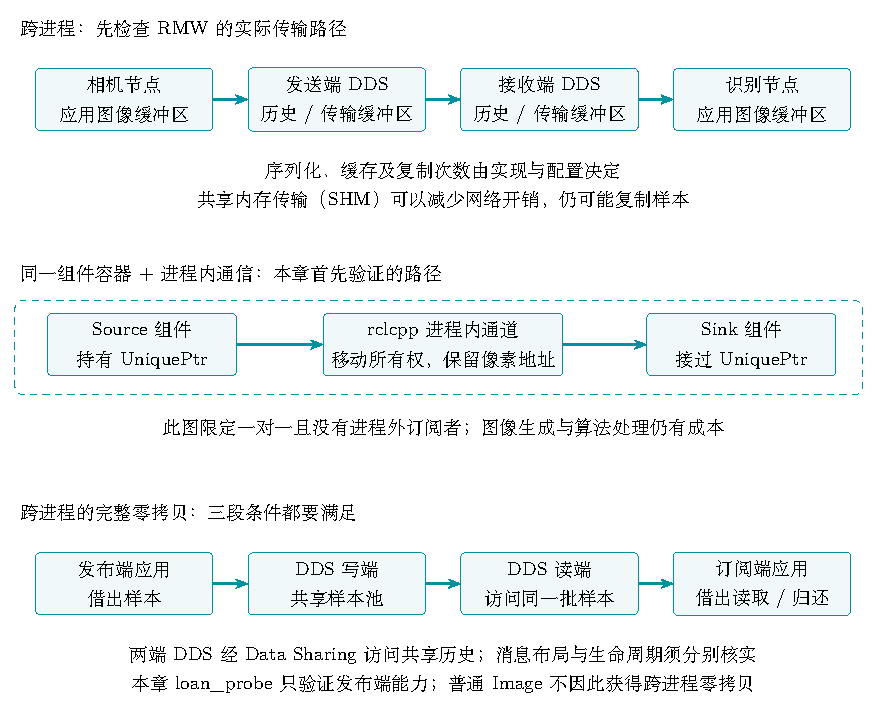
\includegraphics[width=0.97\textwidth]{images/ros2_image_paths_revised.pdf}
\caption{三种数据路径：区分进程内传递、共享内存传输与完整的跨进程零拷贝}
\label{fig:ros2-image-paths}
\end{figure}

图\ref{fig:ros2-image-paths} 中间一行是我们先动手验证的路径。\textbf{组件（component）}是可装载的节点实现，\textbf{组件容器（component container）}是承载它们的进程。组件不是一种新消息类型，也不会因为装到一起就自动启用进程内通信。两端要接收并使用 \texttt{NodeOptions}，启用 \nolinkurl{use_intra_process_comms}，并选择合适的消息所有权接口。

发布者创建 \texttt{UniquePtr}，通过 \texttt{publish(std::move(msg))} 交出消息，唯一订阅者用同类指针接过它。\texttt{std::move} 表达“可以转移所有权”，本身不保证任意传输路径零拷贝。实际能否直接交接，要看 \texttt{rclcpp} 的布局和订阅条件。交出以后不要继续访问原消息；接收端也不能留下一个裸指针，却让持有消息的智能指针先销毁。

\begin{note}
先前进入的 Distrobox、以及 Docker/Podman 的容器属于运行环境：它们管理文件系统、进程与设备等资源。ROS2 组件容器属于节点部署方式：它把组件放进同一个进程。两个节点即使在同一个 Distrobox 内，若分别启动两个进程，也仍不能使用这条 \texttt{rclcpp} 进程内路径。跨系统容器尝试 DDS 共享内存时，还要检查 IPC/共享目录、权限、容量与发现网络；网络能通不代表共享内存能用，GPU 驱动可用也不代表图像传输自动零拷贝。
\end{note}

\paragraph*{一份源码，三种部署}
\begin{example}[合成图像从 Source 交给 Sink]
先用默认的 $64\times48@25\,\mathrm{Hz}$ 跑通，再换成相机的大尺寸负载。项目不需要真实相机，接收端只检查首尾像素并统计回调入口时刻，暂时不做识别。目录如下：
\par\medskip\noindent\begin{minipage}{\linewidth}
\begin{tbash}
image-path-demo/
  package.xml             # 依赖与接口包声明
  CMakeLists.txt          # 消息生成、组件注册和安装
  msg/Frame.msg           # 图像与实验测量元数据
  src/components.cpp     # Source、Sink 两个组件
  src/loan_probe.cpp     # 下一节的借出能力探测
  launch/path.launch.py  # 相同节点的三种布局
  config/fastdds-loan.xml # 下一节的显式配置
  compare.py             # 独立进程组运行并保存统计
\end{tbash}
\end{minipage}\par\smallskip

\texttt{Frame.msg} 给正常的 \texttt{sensor\_msgs/Image} 加一层实验包装，序号、单调时钟和源缓冲区地址都放在包装里。\texttt{Image.header.stamp} 仍是节点时钟下的生成时间，\texttt{frame\_id} 仍表示相机坐标系，不拿它们偷偷塞测试字符串。
\par\medskip\noindent\begin{minipage}{\linewidth}
\lstinputlisting[frame=single,caption={图像包装接口}]{examples/ros2/image-path-demo/msg/Frame.msg}
\end{minipage}\par\smallskip

下面是完整的组件源码。Source 等订阅者出现后，按定时器周期分配并填充像素；完成指定帧数后停止发布。\texttt{sent\_ns} 在填充完成后、调用 publish 前记录，所以延迟统计从这里起算，发送频率则还会受到分配、填充与发送阻塞影响。
\lstinputlisting[frame=single,language=C++,caption={合成图像发布组件与公共定义},firstline=1,lastline=76]{examples/ros2/image-path-demo/src/components.cpp}

Sink 接到消息时记录延迟，检查首尾像素，再在正常退出时输出统计。地址只在源端与接收端 PID 相同、同一帧对应的情况下比较；跨进程的虚拟地址不能用于证明共享了物理内存。\texttt{work\_ms} 是可选的模拟处理耗时，默认 0。
\lstinputlisting[frame=single,language=C++,caption={图像接收组件与组件注册},firstline=77]{examples/ros2/image-path-demo/src/components.cpp}

本实验在同一台 Linux 上，用 \texttt{steady\_clock} 对应的单调时钟比较发送与回调入口时刻；不要直接把这个测法搬到两台未同步时钟的机器。统计也不包含曝光、SDK 采集、图像填充和识别完成时间。实车更关心从采样到结果、再到执行时的图像年龄，后续要继续埋点。

接下来是完整清单与构建规则。清单声明组件库和消息生成依赖；CMake 生成 \texttt{Frame}、链接类型支持，再注册两个组件类。代码末尾的注册宏与 CMake 中的注册函数配合，容器才能按插件名找到类。
\lstinputlisting[frame=single,language=XML,caption={组件实验依赖清单}]{examples/ros2/image-path-demo/package.xml}
\lstinputlisting[frame=single,language=cmake,caption={接口生成、组件注册与安装规则}]{examples/ros2/image-path-demo/CMakeLists.txt}

Launch 文件保持相同 Source/Sink 和 QoS，只改变布局。\texttt{separate} 启动两个组件容器进程；\texttt{same} 把两者装进同一进程但关闭进程内通信；\texttt{intra} 放到同一进程并为两端启用它。这里使用单线程 \texttt{component\_container}，避免线程并发把最小实验变复杂。
\lstinputlisting[frame=single,language=Python,caption={切换组件布局的 Launch 文件}]{examples/ros2/image-path-demo/launch/path.launch.py}

在 Ubuntu 22.04/Humble 环境内操作。下面把教材所在目录保存为 \texttt{BOOK}，替换成你的路径；工作空间使用新目录，已有同名包时换一个目录，避免覆盖。Bash 中的环境脚本按下面写，Zsh 则使用对应的 \texttt{setup.zsh}。
\par\medskip\noindent\begin{minipage}{\linewidth}
\begin{tbash}
source /opt/ros/humble/setup.bash
sudo apt install ros-humble-rmw-cyclonedds-cpp \
  ros-humble-rclcpp-components ros-humble-rosidl-default-generators
BOOK="$HOME/Apps/Tutorial4New"
mkdir -p ~/image_path_ws/src
cp -r "$BOOK/02-专项技术栈/examples/ros2/image-path-demo" \
  ~/image_path_ws/src/image_path_demo
cd ~/image_path_ws
rosdep install --from-paths src --ignore-src -r -y
colcon build --packages-select image_path_demo \
  --cmake-args -DCMAKE_BUILD_TYPE=Release
source install/setup.bash
export ROS_DOMAIN_ID=87
export ROS_LOCALHOST_ONLY=1
export RMW_IMPLEMENTATION=rmw_fastrtps_cpp
ros2 launch image_path_demo path.launch.py mode:=intra
\end{tbash}
\end{minipage}\par\smallskip
预期先出现三条 \texttt{POINTER} 输出，同一帧的 source 与 sink 像素地址相同，\texttt{same\_process=1}；约四秒后出现 \texttt{SOURCE\_DONE 100}。随后按 Ctrl+C 正常结束，查看 \texttt{SOURCE} 与 \texttt{SINK} 汇总：默认小输入应收到 100 帧、\texttt{bad\_frames=0}、\texttt{pointer\_matches=100}。逐帧打印会干扰高速实验，因此项目只打印前三帧及汇总。正常退出用于输出统计，直接强制杀死进程不会得到完整记录。

还可以在另一个加载相同环境、域和 RMW 的终端执行 \texttt{ros2 component list}，看到同一个 \texttt{/image\_box} 下有两个组件。若提示找不到类，核对两处注册名称、构建结果及工作空间环境；若组件存在但收不到消息，回到域、RMW、话题和 QoS 排查。只改 Launch 的 \texttt{mode:=same} 后重复运行，再改成 \texttt{mode:=separate}，应分别看到同进程的普通通信与两个不同 PID 的通信。\texttt{same} 的地址偶然复用不能证明零拷贝，判断必须结合实际启用选项与所有权路径。

切到小图像自动对照时，先停止手动实验，也停止额外的 echo、录制或显示订阅者。\texttt{compare.py} 会依次运行两种 RMW 与三种布局，给每次启动建立独立进程组，等发布完成并留出接收排空时间，再正常关闭这些进程。它清除所测进程里的 DDS 调优变量，不改你的启动文件。
\par\medskip\noindent\begin{minipage}{\linewidth}
\begin{tbash}
cd ~/image_path_ws
python3 src/image_path_demo/compare.py \
  --output /tmp/image-path-small
\end{tbash}
\end{minipage}\par\smallskip
输出目录必须尚不存在；再次运行时换一个名字。里面的 \texttt{results.json} 保存统计，各轮 \texttt{.log} 保留原始输出，\texttt{environment.json} 记录测量口径。参数的一般形式是 \texttt{--width 宽 --height 高 --channels 通道数 --rate 频率 --frames 帧数}；通道数本例只支持 1 与 3，分别对应 mono8 与 bgr8。\texttt{--repeat} 指定重复次数，\texttt{--modes} 可只选择一种布局，\texttt{--domain} 应选一个没有其他实验占用的域。
\end{example}

\paragraph*{系统容器部署：运行环境和共享资源一起检查}
Ubuntu 22.04 的 Distrobox 让我们在同一台主机上保持 Humble 的依赖环境；NVIDIA 支持则把匹配宿主驱动的用户态库与设备接进来。主机负责内核驱动，不要为了容器里的 ROS2 再装一套不匹配的内核驱动。组件容器可以运行在这个环境内，二者是可以同时使用的部署层次。

\begin{example}[进入环境后先确认资源边界]
下面第一条在宿主终端执行，后面的命令在容器内执行。已有 \texttt{ubuntu2204} 环境时直接进入；名称不同时换成自己的。普通 Ubuntu 教学机可以直接检查后面的环境与资源。
\par\medskip\noindent\begin{minipage}{\linewidth}
\begin{tbash}
distrobox enter ubuntu2204
echo "$ROS_DISTRO"
df -h /dev/shm
ls -l /dev/nvidia0 /dev/nvidiactl
nvidia-smi
\end{tbash}
\end{minipage}\par\smallskip
环境加载后应是 humble；为空时先加载适合当前 Shell 的环境脚本。\texttt{df} 检查共享内存挂载的可用容量，设备与 nvidia-smi 检查 NVIDIA 设备/驱动是否可见；没有 NVIDIA 时跳过后两条，按你的 GPU 平台检查。设备可见不代表本例用上了 GPU，本例是 CPU 图像通信测试。

系统容器的网络、IPC 模式和共享目录还需从实际部署配置核对。当前教学 Distrobox 共享宿主网络与 IPC，共享内存挂载约 32 GiB；其他 Podman/Docker 容器可能有独立命名空间与较小容量，不能照抄这个结果。BGR8 的几 MB 样本再乘历史深度、端点和工作缓冲，可能很快超出默认资源预算。遇到共享内存分配失败或传输回退时，先确认路径、权限、容量和实现配置；发现不通则先查域与网络。跨系统容器的完整共享样本交付须另行验证。
\end{example}

\paragraph*{组件化省下复制，也改变故障边界}
同一个进程里的相机、预处理与识别组件共享故障命运：其中一个崩溃，整个容器可能一起退出。单线程执行器中，一个耗时回调还会推迟其他回调。改用多线程容器 \nolinkurl{component_container_mt} 时，也要安排回调组（callback group）并检查共享数据；多线程既不自动保证并行，也不自动解决竞争条件。

因此，你可以先把需要传大图像的近邻节点组合起来，把控制、监控等职责按故障隔离要求拆开。多个订阅者也要考虑所有权：一份消息不能同时独占地交给两个 \texttt{UniquePtr} 接收者，可能产生复制；只读共享则要明确生命周期。外部录制、可视化或网络订阅者加入后，还可能触发额外的中间件发送。实验里暂时不加它们，部署时再逐个补测。

使用 OpenCV 时，\texttt{cv::Mat} 可以视图方式引用已有像素，也可能通过 \texttt{clone}、颜色转换等操作新建数据；要逐处核对。进程内消息直接交接之后又立刻 clone，一样会把大图像再搬一遍。CPU 图像交给 GPU 推理的边界也单独检查，不能把“机器有显卡”算成零拷贝证据。

\begin{exercise}
\label{ex:v2-ros-components}
用同一份源码依次运行 \texttt{intra}、\texttt{same}、\texttt{separate}，记录组件容器、PID 是否相同和前三帧的地址。解释为什么只有开启进程内路径并转移所有权的条件与地址记录一起，才能支持本例的像素传递结论。再检查运行环境的共享内存与 GPU 设备可见性，说明同一个 Distrobox 内启动两个独立节点是否满足进程内通信条件，以及哪些 GPU 传输边界还没被本例验证。
\end{exercise}

\subsubsection{借出消息：向中间件借一块内存}
\label{sec:ros2-loaned-messages}
前面由应用创建消息，再在进程内转移所有权。\textbf{借出消息（loaned message）}换了一个内存来源：发布者向中间件借样本缓冲区，把内容直接写进去，发布后交还控制权。如果支持条件满足，就能减少应用与中间件之间的一次复制或分配。它与组件化相关，却不是同一个开关，也不要求节点一定在同一个进程。

这里最容易踩坑的是 \texttt{borrow\_loaned\_message()} 的回退行为。底层不支持时，\texttt{rclcpp} 可以使用本地分配器继续运行；“借到了一个 C++ 对象”不能证明对象来自中间件。要先查询这个发布者的 \texttt{can\_loan\_messages()}，再记录实际 RMW、类型与配置。

\begin{example}[用 Float64 和 Image 探测借出能力]
沿用刚才的工程，完整程序如下。\texttt{Float64} 是简单固定大小类型；普通 \texttt{Image} 内含可变长像素数组与字符串。探测程序同时查询两者，再借出并发布一个值为 42 的 Float64。它只验证发布端借出和发布调用，不把订阅端或跨进程零拷贝算作已经验证。
\par\medskip\noindent\begin{minipage}{\linewidth}
\lstinputlisting[frame=single,language=C++,caption={借出能力与本地分配回退探测}]{examples/ros2/image-path-demo/src/loan_probe.cpp}
\end{minipage}\par\smallskip

在本章的 Humble/Fast DDS 实现中，固定类型还需要启用 Data Sharing，不能照搬“默认就能借出”的结论。项目给出一份显式配置，设置同步发布、可扩展的预分配历史，以及两端 Data Sharing 自动选择；它不强迫不支持的图像类型使用共享样本。
\par\medskip\noindent\begin{minipage}{\linewidth}
\lstinputlisting[frame=single,language=XML,caption={借出探测用的 Fast DDS 配置}]{examples/ros2/image-path-demo/config/fastdds-loan.xml}
\end{minipage}\par\smallskip

先从没有遗留 DDS 配置的终端开始，确认当前工作目录没有 \nolinkurl{DEFAULT_FASTRTPS_PROFILES.xml}，加载环境后依次运行。变量仅写在一条命令前，只影响那次进程；路径通过已安装包获取。
\par\medskip\noindent\begin{minipage}{\linewidth}
\begin{tbash}
source /opt/ros/humble/setup.bash
cd ~/image_path_ws
source install/setup.bash
export ROS_DOMAIN_ID=88
export ROS_LOCALHOST_ONLY=1
unset ROS_DISABLE_LOANED_MESSAGES
unset FASTRTPS_DEFAULT_PROFILES_FILE RMW_FASTRTPS_USE_QOS_FROM_XML
RMW_IMPLEMENTATION=rmw_fastrtps_cpp \
  ros2 run image_path_demo loan_probe
PROFILE="$(ros2 pkg prefix --share image_path_demo)/config/fastdds-loan.xml"
RMW_IMPLEMENTATION=rmw_fastrtps_cpp \
  FASTRTPS_DEFAULT_PROFILES_FILE="$PROFILE" \
  RMW_FASTRTPS_USE_QOS_FROM_XML=1 \
  ros2 run image_path_demo loan_probe
RMW_IMPLEMENTATION=rmw_cyclonedds_cpp \
  ros2 run image_path_demo loan_probe
RMW_IMPLEMENTATION=rmw_fastrtps_cpp \
  FASTRTPS_DEFAULT_PROFILES_FILE="$PROFILE" \
  RMW_FASTRTPS_USE_QOS_FROM_XML=1 ROS_DISABLE_LOANED_MESSAGES=1 \
  ros2 run image_path_demo loan_probe
\end{tbash}
\end{minipage}\par\smallskip
本章验证环境下，四轮 \texttt{LOAN} 输出的 \texttt{float64/image} 分别为 $0/0$、$1/0$、$0/0$、$0/0$。返回 0 的轮次会提示使用本地分配器；这是可用的回退路径。若你的结果不同，先记录版本与配置，再核对所用实现，不能为了让结果“像教材”而把 true 写死。
\end{example}

\paragraph*{Zenoh 的共享内存与借出 API 分开看}
Zenoh 同样能优化本机序列化数据的传输。项目记录器的 \texttt{--zenoh-shm} 会为节点与路由器显式启用共享内存及传输优化；本章使用的默认配置关闭这一功能。它可以在普通发布路径下工作，不要求应用先调用借出 API。本章 Zenoh 0.1.9 的 Float64/Image 探测在关闭和开启共享内存时均为 0/0，发布调用通过本地分配器回退完成。因此，\texttt{can\_loan\_messages()} 为 false 与“传输层可以使用共享内存”并不矛盾；普通 Image 仍有对象分配、填充及序列化/反序列化边界，不能把传输优化说成相机到算法的完整零拷贝。

先按第\ref{sec:ros2-rmw-selection}节启动自己的 Zenoh 路由器。在已加载 Humble 和组件工程的第二个终端运行发布端探测：
\par\medskip\noindent\begin{minipage}{\linewidth}
\begin{tbash}
RMW_IMPLEMENTATION=rmw_zenoh_cpp \
  ros2 run image_path_demo loan_probe
ZENOH_CONFIG_OVERRIDE='transport/shared_memory/enabled=true' \
  RMW_IMPLEMENTATION=rmw_zenoh_cpp \
  ros2 run image_path_demo loan_probe
\end{tbash}
\end{minipage}\par\smallskip
这里只有一个发布者，测的是借出接口，没有建立订阅端共享样本实验；不能拿这两次调用验证共享内存交付。结束后正常停止自己的路由器。

\begin{example}[开了共享内存，也要检查有没有回退]
在同一个工程里，先看容量与进程资源限制：
\begin{tbash}
df -h /dev/shm
ulimit -l
\end{tbash}
本轮容器的共享内存空间约 32 GiB，锁定内存上限却只有 8192 KiB，即 8 MiB。所用 Zenoh 会锁定共享段，默认 48 MiB 池超过这个限制，日志出现 \texttt{Error creating lazy ShmProvider} 与 \texttt{OS error 12}；消息仍能交付，所以“收到 1000 帧”不能证明共享路径生效。不要只看到 \texttt{enabled=true} 就宣布优化成功。

本实验改用 6 MiB 池重测，完整参数见第\ref{sec:ros2-image-measurement}节。这个设置足够放下一帧约 4.67 MB 的 BGR8，但可容纳的在途大样本很少；它是当前环境的演示条件，实际系统仍需按并发量规划池容量与资源限制。不要照搬 6 MiB 到所有相机。日志还要检查分配失败与回退；共享池创建成功也不能证明整条链路完全没有复制。
\end{example}

\paragraph*{为什么普通 Image 不能直接套用这个结论}
固定长度、可直接映射的 plain 消息布局适合共享样本池；字符串与可变长数组通常不能直接放到这种借出路径里。即使给序列规定一个最大长度，也不等于自动满足 plain 布局。\texttt{Image} 在上面的探测中返回 false，包装了它的 \texttt{Frame} 也不能靠外面多加几个字段就变成固定布局。

真要做跨进程大图像借出，需要设计并验证合适的固定布局或专门传输层，处理内存池容量、分辨率变化、两端生命周期与工具兼容性，还要核对生成的类型支持；不能随手把几 MB 的大数组放在栈上就宣称完成优化。对当前标准图像接口，先采用已验证的组件进程内路径，是更容易保持工具兼容与教学清晰的起点。

\paragraph*{共享内存传输不等于完整零拷贝}
共享内存传输（SHM transport）主要改变 DDS 的传输通道，样本仍可能复制到传输缓冲区再从中取出。Data Sharing 让读写端访问共享样本历史；若应用两端仍然复制到自己的对象里，也还没有消除整条路径的复制。图\ref{fig:ros2-image-paths} 最后一行需要发布端借出、共享样本交付和订阅端借出读取一起成立。

订阅端借出还涉及实现支持与样本有效期限制；本章不通过全局设置 \nolinkurl{ROS_DISABLE_LOANED_MESSAGES=0} 去强行开启它。普通订阅收到 42，最多证明这个值被交付，不能证明接收端从共享池直接借读。发布成功后，原借出对象已不归应用继续读写；没发布的借出对象也要按接口归还，\texttt{rclcpp::LoanedMessage} 的生命周期管理帮助你处理这一点。

这几项分别对应 \href{https://github.com/ros2/rclcpp/blob/humble/rclcpp/include/rclcpp/loaned_message.hpp}{Humble 的借出与回退实现}、\href{https://github.com/ros2/rmw_fastrtps/blob/humble/rmw_fastrtps_cpp/src/publisher.cpp}{发布者借出条件}，以及 \href{https://fast-dds.docs.eprosima.com/en/v2.6.11/fastdds/use_cases/zero_copy/zero_copy.html}{Fast DDS 的完整零拷贝条件}。查资料时分清 DDS 库具备的能力、RMW 暴露的能力和你的节点实际使用的路径。

\begin{exercise}
\label{ex:v2-ros-loans}
保存四轮 DDS loan\_probe 的原始输出，找出真正从中间件借出 Float64 的轮次；再比较 Zenoh 关闭与开启共享内存的借出输出。解释 Image 返回 false、程序却仍能运行的原因，以及为什么这份记录不能证明跨进程图像已经完整零拷贝。写出借出对象发布后必须遵守的所有权规则。
\end{exercise}

\begin{conclusion}
\begin{itemize}
\item RMW 选择决定通信实现，QoS 决定交付与历史策略；两者都不能补足不足的处理能力。
\item ROS2 组件容器安排节点的进程边界，Distrobox 安排运行环境；同进程还需启用进程内通信并管理所有权。
\item 进程内直接交接、DDS 共享内存传输、Data Sharing、Zenoh 传输优化与借出消息分别解决不同边界；零拷贝结论必须指出范围。
\item 借出 API 可以回退。先看能力、消息布局与配置，再看实际缓冲区和生命周期。
\end{itemize}
\end{conclusion}

\subsubsection{把负载升到 250 Hz，再看图像有没有变旧}
\label{sec:ros2-image-measurement}
现在小图像已跑通，我们把合成负载改成 $1440\times1080$ 的 BGR8。尺寸与目标频率来自前面的相机场景，像素由内存生成；这次测试没有接相机、转换 Bayer 或运行识别算法。目标 250 Hz 是定时器请求，不是程序预先保证的实测结果。

\begin{example}[重复三轮，保存吞吐与延迟记录]
先停止手动节点与额外订阅者，在同一个工作空间执行：
\par\medskip\noindent\begin{minipage}{\linewidth}
\begin{tbash}
python3 src/image_path_demo/compare.py \
  --output /tmp/image-path-bgr250 \
  --width 1440 --height 1080 --channels 3 \
  --rate 250 --frames 1000 --repeat 3
\end{tbash}
\end{minipage}\par\smallskip
每种组合正常发完 1000 帧后留两秒接收排空时间；程序输出实际发送/接收频率、接收比例与 P95。统计源码见 \texttt{compare.py}，参数和计时点已在环境记录中写明。出现未完成、缺少正常退出统计或像素检查失败时，脚本会报错并保留日志，不会把失败轮次填成零延迟。

% DDS: bgr250-1440x1080 的 18 轮；Zenoh: 本轮 bgr250 的 9 轮与 shm-6mib 的 3 轮。
\begin{table}[htbp]
\centering
\small
\caption{同机合成 BGR8 大图像对照，每项为三轮数值的中位数}
\label{tab:ros2-image-results}
\begin{tabular}{llrrrr}
\toprule
RMW & 布局 & 发送 / Hz & 接收 / Hz & 接收比例 & P95 / ms\\
\midrule
Fast DDS & separate & 250.0 & 87.5 & 34.7\% & 2.445\\
Fast DDS & same & 250.0 & 250.2 & 100.0\% & 0.968\\
Fast DDS & intra & 250.0 & 250.0 & 100.0\% & 0.042\\
Cyclone DDS & separate & 250.0 & 249.6 & 99.7\% & 3.580\\
Cyclone DDS & same & 250.1 & 250.2 & 100.0\% & 0.959\\
Cyclone DDS & intra & 250.0 & 250.0 & 100.0\% & 0.031\\
\midrule
Zenoh & separate & 250.1 & 250.3 & 100.0\% & 3.243\\
Zenoh & same & 250.0 & 250.2 & 100.0\% & 0.913\\
Zenoh & intra & 250.0 & 250.0 & 100.0\% & 0.029\\
Zenoh + SHM & separate & 250.0 & 250.4 & 100.0\% & 1.822\\
\bottomrule
\end{tabular}
\end{table}
这组 $1440\times1080$ 的 BGR8 数据在 2026 年 10 月 3 日的 Ubuntu 22.04/Humble Distrobox 中测得，主机为 i7-12700H，系统识别约 62.6 GiB 内存；Fast DDS 与 Cyclone DDS 的 RMW 分别为 6.2.10 与 1.3.5，Zenoh RMW/vendor 均为 0.1.9，Fast DDS 为 2.6.12，rclcpp 为 16.0.21。容器共享宿主网络和 IPC，测试清除 DDS/Zenoh 调优变量，深度 5、best\_effort、没有外部订阅者、没有算法工作。每轮发送 1000 帧，再留两秒排空；表中各项分别取中位数，P95 未跨轮合并样本。

Fast DDS 的 separate 接收比例三轮为 34.7\%、35.9\%、18.1\%；Cyclone DDS 为 99.7\%、99.7\%、99.8\%。在这个默认配置与输入下，后者交付比例更高；Fast DDS 已收到样本的 P95 较低，不能抵消丢掉的大量帧。两种 DDS 的 same 与 intra 共 12 轮都完整收到 1000 帧，intra 的像素地址记录全部匹配。

这些记录支持我们优先检查进程布局与所有权路径，也提醒我们继续核对配置，而不是给中间件排一个永久名次。

Zenoh 的三种布局各重复三轮，默认关闭共享内存，九轮均收到 1000 帧。它的路由器只监听本机独立端口，同机 peer 直接连接；本轮结果不能代替跨主机、无线或多机器人链路实测。表中最后一行是另外三轮显式配置：开启 Zenoh 共享内存并使用 6 MiB 池，不能与默认项混为一种配置。其 P95 中位数约 1.822 ms，默认 separate 约为 3.243 ms；进程内路径仍更短，说明传输优化与应用层所有权交接解决的边界不同。

最初用默认 48 MiB 池打开共享内存时，容器的 8 MiB 锁定内存限制导致分配失败。那三轮虽然也完整交付，却出现共享池错误，不能算作成功的 SHM 对照；回退记录另存，未放进上表。6 MiB 池的重测没有出现这个分配错误；后续仍要核对在途样本与回退，不能凭配置开关推断每帧路径或完整零拷贝。

小图像的 same 模式中，还出现过 50 帧里 49 次源/接收像素地址数值相等：它没有开启进程内通信，分配器复用地址造成了这种现象。因此，地址记录必须与启用选项、所有权和生命周期一起判断。

逐轮数据、原始日志与测量边界保存在仓库 \path{docs/revision/evidence/ros2-image-path-20261003-runtime/}。Zenoh 追加记录保存在 \path{docs/revision/evidence/ros2-zenoh-20261003-runtime/}。这些是合成像素通信数据，不是相机采集到识别完成的实测；CPU/GPU 转换与跨系统容器的共享样本路径也未由此验证。


观察时先问：Source 是否真的接近 250 Hz？如果没有，接收端频率低可能来自源端分配、发送阻塞或同进程回调争用；如果 Source 接近 250 Hz，接收比例却很低，才继续查交付与接收瓶颈。P95 低也要配合接收比例读，不能只拿已经收到的少数新帧做结论。\texttt{same} 与 \texttt{intra} 都有一个单线程容器，\texttt{separate} 有两个容器进程，所以对照同时体现部署布局的变化；不能把全部差值都算成某一种 DDS 内部复制的耗时。

记录器还保存本实验进程组的累计 CPU 秒和进程 RSS 之和。CPU 包括发现、加载与排空，不能直接当作稳态利用率；RSS 之和可能重复计算共享页，不能直接当作实际物理内存用量。真正选型时再分段测量、重复并改变实验顺序，必要时采用跟踪工具定位具体复制或等待位置。
\end{example}

\Needspace{9\baselineskip}
\paragraph*{把 Zenoh 加进大图像对照}
上面的默认命令保留两种 DDS。安装 Zenoh 后，保持相同图像、QoS 和三种布局，另用新目录运行：
\par\medskip\noindent\begin{minipage}{\linewidth}
\begin{tbash}
python3 src/image_path_demo/compare.py \
  --output /tmp/image-path-zenoh-bgr250 --rmws rmw_zenoh_cpp \
  --width 1440 --height 1080 --channels 3 \
  --rate 250 --frames 1000 --repeat 3
\end{tbash}
\end{minipage}\par\smallskip
需要一次调度三个实现时，用 \texttt{--rmws} 同时列出三种 RMW。记录器仍使用自己的路由器与本机端点，默认关闭 Zenoh 共享内存，避免把改变传输配置与改变 RMW 混成一个变量。

然后只保留两个进程，显式打开共享内存，并记录前面检查过的池容量：
\par\medskip\noindent\begin{minipage}{\linewidth}
\begin{tbash}
python3 src/image_path_demo/compare.py \
  --output /tmp/image-path-zenoh-shm \
  --rmws rmw_zenoh_cpp --modes separate --zenoh-shm \
  --zenoh-shm-pool-mib 6 \
  --width 1440 --height 1080 --channels 3 \
  --rate 250 --frames 1000 --repeat 3
\end{tbash}
\end{minipage}\par\smallskip
这是第二项独立对照，不能混入默认配置的结果。记录器保存共享内存开关、池容量、端口及路由器日志；检查 \texttt{zenoh\_shm\_provider\_error} 与原始日志，再读吞吐和延迟。资源限制、历史深度和在途样本都可能改变结果；即使本轮完整交付，也要继续测算法、实际相机与网络。

\paragraph*{故意让识别变慢一次}
接下来只保留 Fast DDS 的两个进程，把 Sink 的模拟处理设为 8 ms。先用默认小图像观察排队，不让图像大小掩盖处理能力问题：
\par\medskip\noindent\begin{minipage}{\linewidth}
\begin{tbash}
python3 src/image_path_demo/compare.py \
  --output /tmp/image-path-slow \
  --rmws rmw_fastrtps_cpp --modes separate \
  --rate 250 --frames 500 --work-ms 8 --depth 5
\end{tbash}
\end{minipage}\par\smallskip
预期接收处理跟不上到帧节奏，可能丢帧并出现等待；看实际发送频率、接收比例和延迟，不要求输出某个固定帧数。换用 \texttt{--depth 100}，对比丢帧与图像年龄。较深队列可能让更多旧帧被处理，代价是延迟；本例有限帧数可能最终排空，不能把“最后都收完”当作长期稳定。若慢处理需要更久排空，可增大 \texttt{--drain-seconds}，并把这个条件记录下来。

本次小图像实测中，两轮 Source 都接近 250 Hz，Sink 约为 122 Hz。深度 5 收到 249/500 帧，P95 约 20.0 ms；深度 100 收到 344/500 帧，P95 约 746.6 ms，两轮都使用两秒排空。较深的队列让这一轮收到了更多帧，也让已经收到的旧帧等得更久。数值是这次实验的结果，后续按自己的日志核对。

对串行的长期 8 ms 阶段，应该减少工作量、降采样、只处理最新帧，或设计可验证的并行流水线。零拷贝会减少搬运成本，却不能省掉算法本来需要的计算。图像容器还要配好外部观测边界：250 Hz 图像没必要全速送给 GUI，可以专门降频/缩小后输出给显示与录制节点。

\begin{exercise}
\label{ex:v2-ros-image-slow}
运行深度 5 和 100 的慢处理对照，记录实际发送频率、接收比例、P95 和排空时间。根据记录解释吞吐、丢帧和图像年龄的关系；再给相机到识别的主链路与降频可视化支路画一份部署方案，说明组件组合、进程隔离和 RMW 的选择依据。
\end{exercise}
